\chapter{Задачи с аналитическим решением}
\newcommand{\Ip}{I_\text{p}}
\label{chap:problem}

\section{Задача об излучающем шаре}
\label{sec:sphere}

В бесконечной среде с коэффициентом поглощения $\varkappa = \varkappa_1$ с равновесным излучением $\Ip = 0$ находится 
шар из материала с $\varkappa = \varkappa_2$, однородно излучающий с $\Ip = I_0$.
\begin{figure}[ht!]%
\centering%
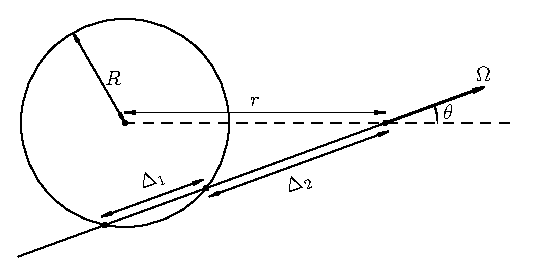
\includegraphics[width=0.5\columnwidth]{box-0}%
\quad%
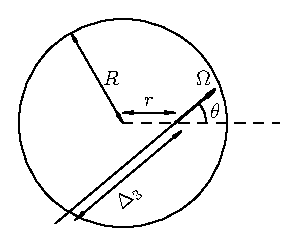
\includegraphics[width=0.27\columnwidth]{box-1}%
\caption{К построению решения уравнения переноса вдоль луча}%
\end{figure}

Переменные, изображенные на рисунке равны:
\begin{gather*}
\Delta_1 = 2\sqrt{R^2 - r^2 \sin^2 \theta}\\
\Delta_2 = r \cos \theta - \sqrt{R^2 - r^2 \sin^2 \theta}\\
\Delta_3 = r \cos \theta + \sqrt{R^2 - r^2 \sin^2 \theta}.
\end{gather*}

Уравнение переноса вдоль луча можно записать в виде
\begin{align*}
\frac{dI(s)}{ds} + \varkappa I = \varkappa \Ip.
\end{align*}

В точке $-\infty$ интенсивность равна нулю, она продолжает не изменяться, пока луч не дойдет до шара. Как только луч окажется в шаре, интенсивность
будет нарастать по закону \mbox{$I_0(1-e^{-\varkappa_2 \Delta s})$}. На выходе из шара интенсивность будет равна 
\mbox{$I_0(1-e^{-\varkappa_2 \Delta_1})$}. Далее, интенсивность снова спадает 
по экспоненциальному закону.
\begin{align*}
I(r,\theta) = I_0
\begin{cases}
1-e^{-\varkappa_2 \left(r \cos \theta + \sqrt{R^2 - r^2 \sin^2 \theta}\right)},&R > r\\
\left(1-e^{-2\varkappa_2\sqrt{R^2 - r^2 \sin^2 \theta}}\right)
e^{-\varkappa_1 \left(r \cos \theta - \sqrt{R^2 - r^2 \sin^2 \theta}\right)},&\theta < \arcsin \frac{R}{r}\\
0,&\text{иначе}
\end{cases}.
\end{align*}
Найдем плотность энергии излучения, поток энергии вдоль радиуса и компоненту $rr$ тензора потока импульса
\begin{align*}
U(r) &= \frac{1}{c} \int\limits I(r,\Omega) d\Omega = \frac{2\pi}{c} \int\limits_0^\pi I(r, \theta) \sin \theta d\theta\\
S_r(r) &= \int\limits \Omega_r I(r,\Omega) d\Omega = 2\pi \int\limits_0^\pi \cos \theta I(r, \theta) \sin \theta d\theta\\
T_{rr}(r) &= \frac{1}{c} \int\limits \Omega_r^2 I(r,\Omega) d\Omega = \frac{2\pi}{c} \int\limits_0^\pi \cos^2 \theta I(r, \theta) \sin \theta d\theta.
\end{align*}
Заменим $\cos \theta = \mu, \sin^2 \theta = 1-\mu^2$. Интегрирование заменится по правилу
\begin{align*}
\int\limits_0^\pi \bullet \sin \theta d\theta = \int\limits_{-1}^1 \bullet d\mu.
\end{align*}
Интенсивность в новых обозначениях примет вид
\begin{align*}
I(r,\mu) = I_0
\begin{cases}
1-e^{-\varkappa_2 \left(\mu r + \sqrt{R^2 - (1-\mu^2)r^2}\right)},&R > r\\
\left(1-e^{-2\varkappa_2\sqrt{R^2 - (1-\mu^2)r^2}}\right)
e^{-\varkappa_1 \left(\mu r- \sqrt{R^2 - (1-\mu^2)r^2}\right)},&\mu > \sqrt{1-\frac{R^2}{r^2}}\\
0,&\text{иначе}
\end{cases},
\end{align*}
а $U, S_r$ и $T_{rr}$ соответственно
\begin{align*}
U(r) &= \frac{2\pi}{c} \int\limits_{-1}^{1} I(r, \mu) d\mu\\
S_r(r) &= 2\pi \int\limits_{-1}^1 \mu I(r, \mu) d\mu\\
T_{rr}(r) &= \frac{2\pi}{c} \int\limits_{-1}^1 \mu^2 I(r, \mu) d\mu
\end{align*}
Также можно рассмотреть тензор направленности излучения $\mathbb D = \frac{1}{U} \mathbb{T}$. В случае изотропного излучения $\hat D = \frac{1}{3}\mathbb I$

\begin{figure}[ht!]%
\centering
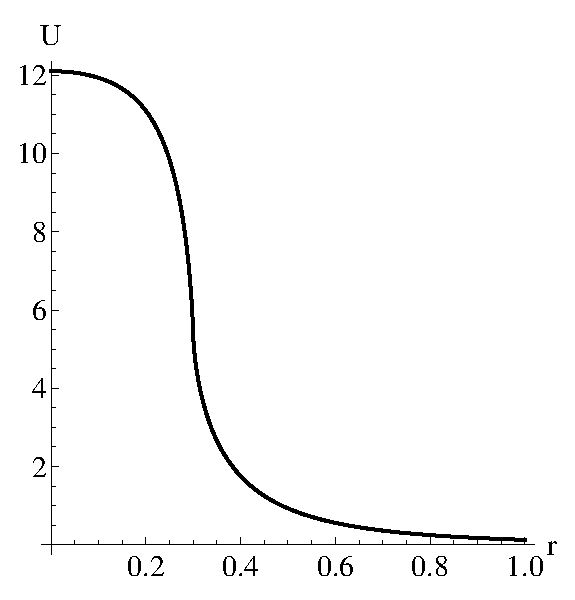
\includegraphics[width=.3\columnwidth]{U}\quad%
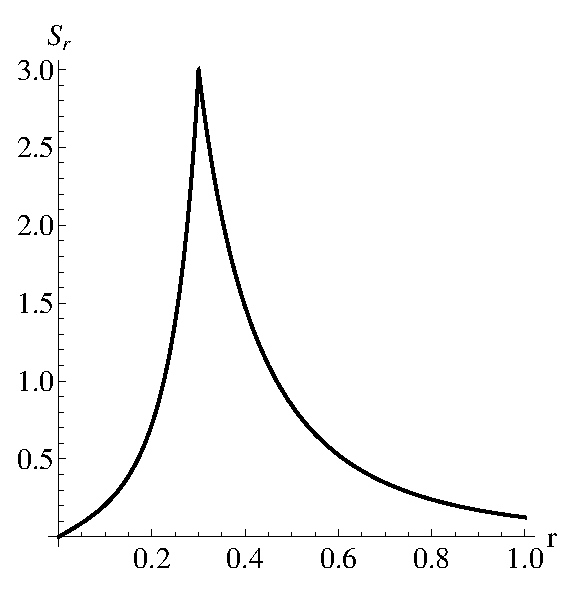
\includegraphics[width=.3\columnwidth]{S.eps}\quad%
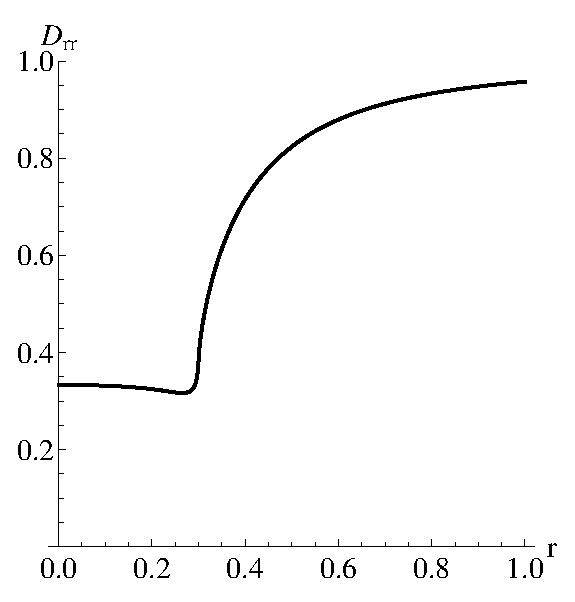
\includegraphics[width=.3\columnwidth]{Drr}%
\caption{Графики плотности энергии, потока энергии и направленности излучения при $R = 0.3, I_0 = 1, c = 1, \varkappa_1 = 1, \varkappa_2 = 11$}%
\end{figure}

\section{Задача о двух полупространствах (задача Милна)}
\label{sec:milne}

Пространство при $x < 0$ заполнено веществом с коэффициентом поглощения $\varkappa_1$ и интенсивностью равновесного излучения $\Ip = I_1$,
а при $x \geq 0$ --- веществом с коэффициентом поглощения $\varkappa_2$ и интенсивностью равновесного излучения $\Ip = I_2$.

\begin{figure}[ht!]%
\centering
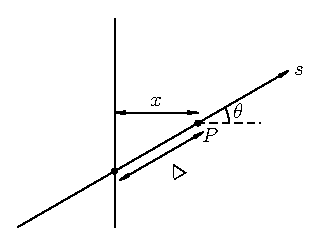
\includegraphics[height=2in]{half-0}%
\caption{К определению интенсивности из уравнения вдоль луча}%
\label{pic:halfspace}%
\end{figure}
Для определенности будем искать $I$ при $x > 0$. 
Величина $\Delta$ на рисунке равна $\frac{x}{\cos \theta}$. Запишем уравнение переноса вдоль луча
\begin{equation*}
\frac{dI(s)}{ds} + \varkappa I = \varkappa \Ip.
\end{equation*}
Обозначим $\mu = \cos \theta$. При $\mu > 0$ интенсивность в $-\infty$ равна равновесной интенсивности в левой области $I_1$.
После пересечения плоскости $x = 0$ решение по экспоненциальному закону $I_1 + (I_2 - I_1) (1 - e^{-\varkappa_2 s})$
стремится к равновесному излучению в правой области. При $\mu \leq 0$, интенсивность равна равновесной интенсивности в правой области $I_2$:
\begin{equation*}
I(x, \mu) = \begin{cases}
I_2 + (I_1 - I_2) e^{-\varkappa_2 \Delta}, &\,\mu > 0\\
I_2 , &\,\mu \leq 0
\end{cases}
\end{equation*}
Аналогично предыдущей задаче,
\begin{align}
U &= \frac{2\pi}{c} \int\limits_{-1}^1 I(x, \mu) d\mu\\
S_x &= 2\pi \int\limits_{-1}^1 \mu I(x, \mu) d\mu\\
T_{xx} &= \frac{2\pi}{c} \int\limits_{-1}^1 \mu^2 I(x, \mu) d\mu
\end{align}
Интегрируя, получаем
\begin{align}
U &= \frac{4\pi}{c} I_2 + \frac{2\pi}{c}(I_1 - I_2)\int\limits_0^1 e^{-\frac{z}{\mu}} d\mu = \nonumber\\
&=\frac{4\pi}{c} I_2 + \frac{2\pi}{c}(I_1 - I_2)\left(e^{-z} + z 
\operatorname{Ei}(-z)\right)\\
S_x &= 2\pi (I_1 - I_2)\int\limits_{0}^1 \mu e^{-\frac{z}{\mu}} d\mu = \nonumber\\
&= \pi (I_1 - I_2) \left((1 - z)e^{-z} - z^2
\operatorname{Ei}(-z)\right)\\
T_{xx} &= \frac{4\pi}{3c}I_2 + \frac{2\pi}{c} (I_1 - I_2)\int\limits_{0}^1 \mu^2 e^{-\frac{z}{\mu}} d\mu = 
\nonumber\\
&= \frac{4\pi}{3c}I_2 + \frac{\pi}{3c} (I_1 - I_2)\left((2 - z + z^2)e^{-z} + z^3 \operatorname{Ei}(-z)\right),
\end{align}
где $z = \varkappa_2 x$ --- оптическое расстояние от границы до точки $x$. Решения при $x < 0$ поулчаются
заменой первой среды на вторую и $z$ на $-z$.
\begin{figure}[ht!]%
\centering
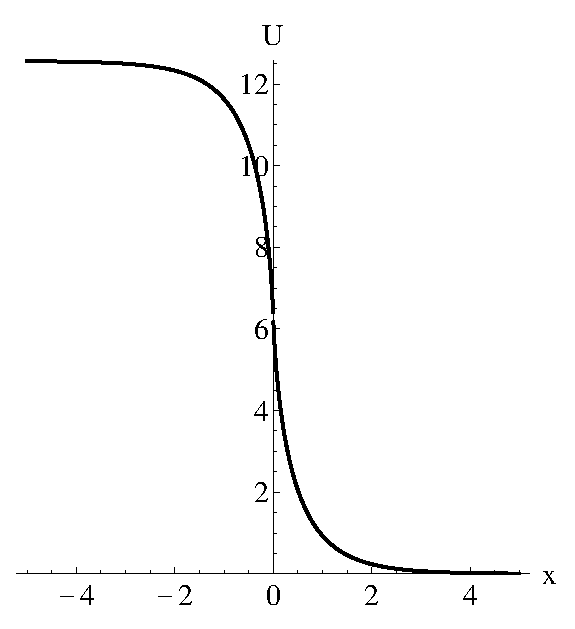
\includegraphics[width=.3\columnwidth]{U2}\quad%
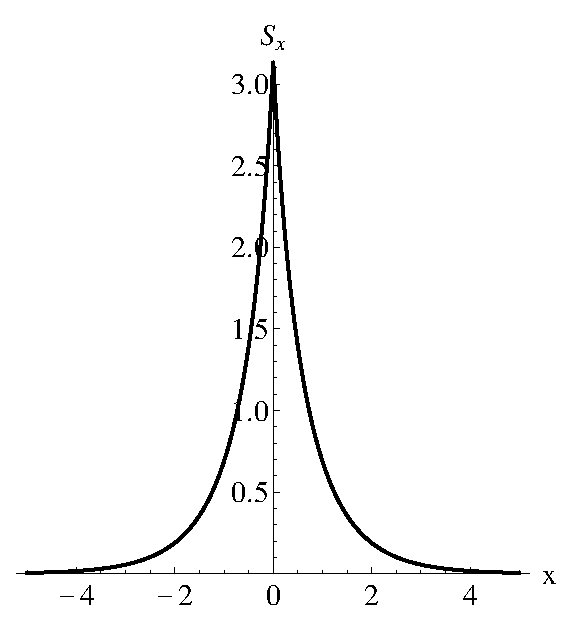
\includegraphics[width=.3\columnwidth]{S2}\quad%
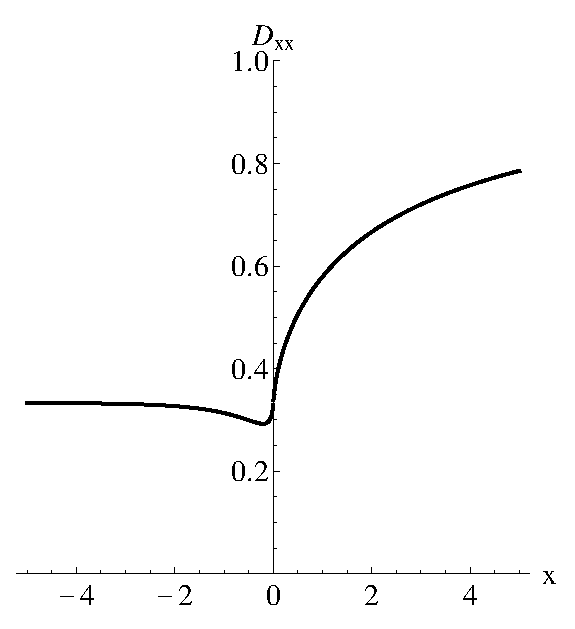
\includegraphics[width=.3\columnwidth]{D2xx}%
\caption{Графики плотности энергии, потока энергии и направленности излучения при $I_2 = 0, I_1 = 1, c = 1$
в зависимости от оптического расстояния от границы}%
\end{figure}
